\section{Harp}
\begin{figure}[htbp]
\centering
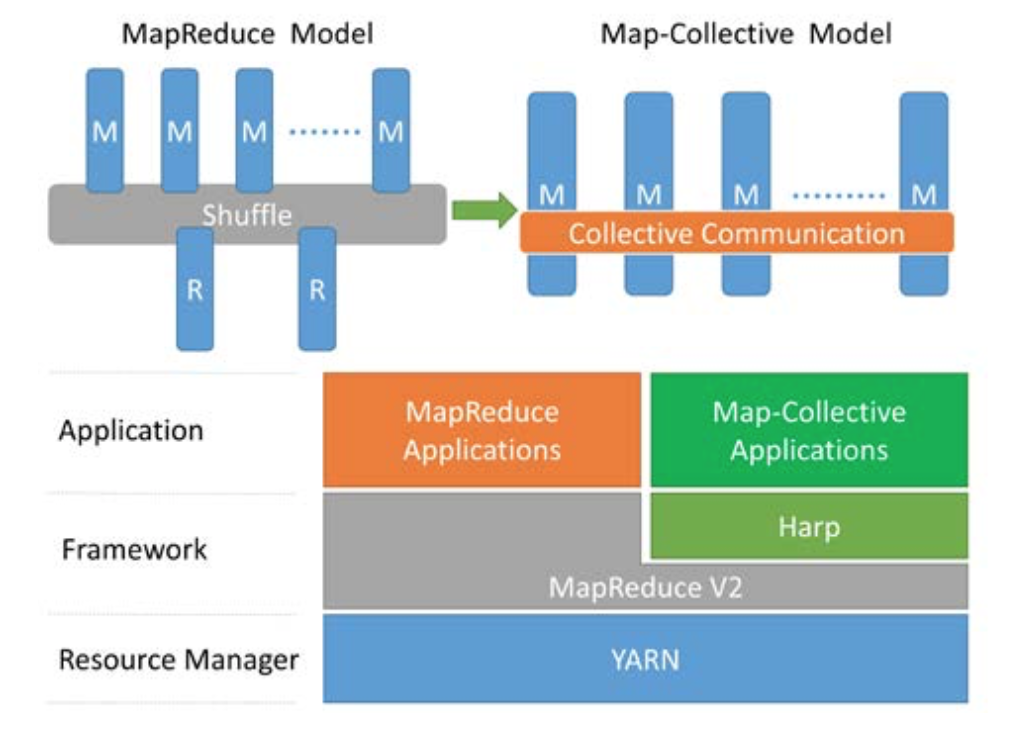
\includegraphics[width=3.0in]{image/Harp-structure.png}
\caption{Parallelism and Architecture of Harp}
\label{Harp}
\end{figure}

Harp provides collective communication library to Hadoop. It also provides associated data abstraction. Based on Hadoop, we can convert MapReduce model into Map-Collective model with the use of Harp. It is also possible to enable efficient in-memory communication, which is one of the greatest advantage Harp produces. When running iterative algorithms, runtime depends largely on communication operations arise  by information updating of each loop. Harp is therefore highly recommended because of its high speed of extracting data from cache. There is no doubt that implementing machine learning algorithms on Hadoop is an efficiency and high performance way. However, Harp works especially well on iterative models since its communication is based on memory while Hadoop is based on disk. Too many I/Os will largely increase runtime. With the implementation of Harp, we can reach high performance of algorithms and reduce runtime. Upon this, we have parallel processes cooperate through collective communication for efficient data processing. 

Benefits from Harp are plenty. When doing communication in MapReduce, the "reduce-gather-broadcast" strategy is applied through on-memory communication in frameworks such as Twister\cite{ekanayake2010twister} and Spark\cite{zaharia2010spark}. 
However, when the data set is large and so do the centroids scales, using "gather-broadcast" is no longer an efficient way. When the work loads on iterative algorithms, communication execution time is even more vital to our consideration. For each iteration, all machines need to communication with other nodes, or by simplification, with the master node. This gives out at least O(MN) operations where M is the number of machines and N is the number of iterations. By then the communication performance contributes lot to the total performance. "Collective Communication" in MPI is a good way which can abstract the communication layer out and therefore provide collective communication abstractions. 
Yet it has limitation supporting high level data abstractions and is not transparency for users. In order to improve this, we use Harp library. We can explain how Harp works as following. Harp works an optimized implementation to provide data abstractions as well as their related communication abstractions. By plugging Harp into Hadoop, we can then convert MapReduce model to Map-Collective model. This enables efficient in-memory communication between Mapper nodes whose tasks can therefore convert messages and finally work across various important data analysis applications.